% !TeX program = xelatex
\documentclass[a4paper,12pt]{article}
\usepackage[left=2.0cm, right=2.0cm, top=2.5cm, bottom=2.0cm]{geometry}
\usepackage{indentfirst}
\usepackage{amsmath, amssymb, amsfonts}
\usepackage{multirow}
\usepackage{graphicx}
\usepackage{xeCJK}
\usepackage{fancyhdr}
\usepackage{verbatim}
\usepackage{algorithm}
\usepackage{algpseudocode}
\usepackage{hyperref}
\usepackage{bm}
\pagestyle{fancy}
\lhead{}
\chead{图形学大作业系统报告}
\rhead{陈劭源(161240004)}
\lfoot{}
\cfoot{}
\rfoot{\thepage}
\setCJKmainfont[BoldFont=SimHei,ItalicFont=KaiTi]{SimSun}
\setCJKmonofont{KaiTi}
\setmainfont{Times New Roman}
\setmonofont{Courier New}
\renewcommand\refname{参考文献}
\graphicspath{{figures/}}

\title{图形学大作业系统报告}
\author{陈劭源(161240004) \\ \href{mailto:sy\_chen@smail.nju.edu.cn}{sy\_chen@smail.nju.edu.cn}}
\date{\today}

\begin{document}
\maketitle

\section{综述}



\section{图元绘制算法介绍}
绘制曲线$f(x,y) = 0$的基本原则是:当$\left|\frac{\mathrm{d}y}{\mathrm{d}x} \big|_{(x_0, y_0)} \right| \leq 1$时,沿$x$轴递进采样画点;当$\left|\frac{\mathrm{d}y}{\mathrm{d}x} \big|_{(x_0, y_0)} \right| > 1$时,沿$y$轴递进采样画点。这样可以保证相邻两个绘制点$(x_i, y_i), (x_{i+1}, y_{i+1})$之间满足$\max\{|x_i - x_{i+1}|, |y_i - y_{i+1}|\} = 1$。

\subsection{直线绘制算法}

\subsubsection{DDA算法}

DDA算法是利用对曲线微分方程积分的方法来绘制曲线的。DDA算法通常用于绘制线段、多边形等,但也可用来绘制非线性曲线\cite{wiki:DDA}。对于直线$y = kx + b$ $(|k| \leq 1)$,DDA算法在每次递增$x$时,对$y$增加$k$,并将取整后的值作为当前绘制点。利用DDA算法绘制线段的伪代码如下:

\begin{algorithm}[htb] 
\caption{DDA画线算法} 
\label{alg:DDA} 
\begin{algorithmic}[1] 
\Require 
线段的两个端点$(x_1, y_1)$, $(x_2, y_2)$。假定$x_1 < x_2, |x_2 - x_1| \geq |y_2 - y_1|$。
\State $y = y_1, k = \frac{y_2 - y_1}{x_2 - x_1}$
\For{$x = x_1$ to $x_2$}
    \State 绘制点 $([x], [y])$
    \State $y = y + k$
\EndFor
\end{algorithmic} 
\end{algorithm}

\subsubsection{Bresenham算法}

Bresenham算法的基本思想是,通过判断下两个绘制点的中点在直线的哪一侧来决定选取哪一个决策点。判断中点在直线哪一侧可以通过维护一个决策变量$\Delta$来实现,而决策变量的维护通常可以利用整数的加减法实现\cite{wiki:Bresenham},因此Bresenham算法比DDA算法更加高效。

对于以$(x_1, y_1), (x_2, y_2)$ (假设$x_1 < x_2, y_1 \leq y_2, |x_1 - x_2| \geq |y_1 - y_2|$)为端点的线段,它的直线方程为

$$ (y - y_1) (x_2 - x_1) = (y_2 - y_1)(x - x_1) $$

故可取决策变量$\Delta(x, y) = 2[(y_2 - y_1)(x - x_1) - (y - y_1)(x_2 - x_1)]$,并根据$\Delta(x_i+1, y_i+0.5)$的符号决定绘制点。当决策变量为正时,递增$y$,否则不递增$y$。决策变量可用以下方式维护:

$$ \Delta(x_i+1, y_i+0.5) = \Delta(x_i, y_i) + 2\Delta y - \Delta x $$
$$ \Delta(x_i+1, y_i+1) = \Delta(x_i+1, y_i+0.5) - \Delta x $$
$$ \Delta(x_i+1, y_i) = \Delta(x_i+1, y_i+0.5) + \Delta x $$

Bresenham算法的伪代码如下

\begin{algorithm}[htb] 
\caption{Bresenham画线算法} 
\label{alg:DDA} 
\begin{algorithmic}[1] 
\Require 
线段的两个端点$(x_1, y_1)$, $(x_2, y_2)$。假定$x_1 < x_2, y_1 \leq y_2, |x_2 - x_1| \geq |y_2 - y_1|$。
\State $y = y_1, \Delta x = x_2 - x_1, \Delta y = y_2 - y_1$
\State $\Delta = -\Delta x$
\For{$x = x_1$ to $x_2$}
	\If{$\Delta \geq 0$}
	\State $y = y + 1, \Delta = \Delta - \Delta x$ 
	\Else
	\State $\Delta = \Delta + \Delta x$
	\EndIf
    \State 绘制点 $(x, y)$
    \State $\Delta = \Delta + 2\Delta y - \Delta x$
\EndFor
\end{algorithmic} 
\end{algorithm}

其中,$[x]$表示$x$舍入至最近的整数。

\subsection{多边形绘制算法}
多边形的绘制算法可以很容易地由直线绘制算法导出。只需要用相应的直线绘制算法依次绘制多边形相邻两个顶点的连线段即可。


\subsection{椭圆绘制算法(中点法)}
中点法绘制椭圆的原理和Bresenham算法十分类似。在中点法中,仍然是通过计算相邻两个可能绘制点的中点在椭圆的哪一侧,从而决定在哪个点上绘制图形。但由于椭圆的特殊性,其绘制方法和直线的绘制方法存在以下差异:

\begin{itemize}
	\item 由于椭圆有两条互相垂直且与坐标轴平行的对称轴,只需要绘制椭圆在任一象限中的图形,就可以通过对称的方式完成整个椭圆的绘制。
	\item 椭圆在任一象限中的图形均存在斜率的变化,因此必须以斜率为1的点作为分界点,对椭圆进行分段绘制。
\end{itemize}
不妨设椭圆中心位于原点。对于两轴半径分别为$r_x,r_y$的椭圆,其方程为$\frac{x^2}{r_x^2} + \frac{y^2}{r_y^2} = 1$,故可取$p(x, y) = x^2r_y^2 + y^2 r_x^2 - r_x^2r_y^2$为决策变量,并根据$p(x+1, y+0.5)$(或$p(x+0.5, y+1)$)的符号决定绘制点。决策点可按以下方式维护:

$$ p(x_i+1, y_i+0.5) = p(x_i, y_i) + 2r_y^2 + r_x^2 $$
$$ p(x_i+1, y_i+1) = p(x_i, y_i) + 2r_y^2 + 2r_x^2 $$
$$ p(x_i+1, y_i) = p(x_i, y_i) + 2r_y^2 $$

算法的伪代码如下:

\begin{algorithm}[htb] 
	\caption{中点法绘制椭圆} 
	\label{alg:DDA} 
	\begin{algorithmic}[1] 
		\Require 
		椭圆的两轴半径$r_x, r_y$。
		\State $p = r_y^2 - r_x^2 ry + rx^2 / 4$
		\State $p_x = 0, p_y = 2r_x^2r_y$
		\State $c_x = 0, c_y = r_y$
		\While{$x = x_1$ to $x_2$}
		\State $c_x = c_x + 1$, $p_x = p_x + 2 r_y^2$ 
		\If{$p < 0$}
		\State $p = p + r_y^2 + px$
		\Else
		\State $c_y = c_y - 1$, $p_y = p_y - 2 r_x^2$
		\State $p = p + r_y^2 + px - py$
		\EndIf
		\State 绘制点 $(x, y)$
		\EndWhile
		\State 交换$x, y$后重复上述步骤。
	\end{algorithmic} 
\end{algorithm}

\subsection{曲线绘制算法}
\subsubsection{Bezier曲线}
Bezier曲线是对给定样本点逼近的常用方法。一般来说,对于$n+1$个样本点(或称控制点),我们可以绘制出$n$阶Bezier曲线。$n$阶Bezier曲线实际上是以$(tx+(1-t))^n$的二项式展开的各项系数为权函数,对样本点进行加权混合的结果,其公式如下:

$$ B(t) = \sum_{i=0}^n \binom{n}{i} P_i t^i (1-t)^{n-i} $$
其中,$P_0, P_1, \cdots, P_n$为样本点。我们可以直接根据公式计算出Bezier曲线在某一点处的坐标,但Bezier曲线还存在一种递推的计算方式:
$$ B_{i, j}(t) = t B_{i-1, j}(t) + (1-t) B_{i-1, j+1}(t) $$
其中,$B_{0, i}(t) = P_i$,$B_{n, 0}(t) = B(t)$。这种计算方式避免了代价较高的浮点数指数运算,虽然时间复杂度由$O(n)$上升为了$O(n^2)$,但在曲线阶数较低时仍有较好的效果。

可以看到,Bezier曲线实际上是由样本点确定的参数曲线,难以表示成显函数的形式,因此之前用于直线、椭圆绘制的中点法等方法不在适用。一种简单的绘制参数曲线的方法是,确定一个步长$\eta$,以$\eta$为间隔等距确定参数$t$的值,然后依次画出曲线上的每个点。然而,参数$\eta$的确定通常是较为困难的,如果$\eta$设置地过小,则会产生很多重复或是多余的点,如果$\eta$设置地过大,则绘制的曲线会产生“缺口”。解决此问题的常用方法是自适应调整$\eta$的值:如果发现相邻两个绘制点重合,则调大$\eta$的值;如果相邻两个绘制点不连续,则调小$\eta$的值。

这里,我们采用一种更加优雅的方法——分治法。注意到,曲线绘制的过程实际上是将曲线上的部分点舍入到平面网格上的整数点,并满足以下条件:

\begin{enumerate}
	\item 对于相邻两个绘制点$\bm{x}_i, \bm{x}_{i+1}$,满足$\|\bm{x}_i - \bm{x}_{i+1}\|_{\infty} = 1$,其中$\| (x, y) \|_{\infty} = \max\{|x|, |y|\}$为$\infty$-范数;
	\item 在满足上述条件的前提下,绘制点的数目尽可能少。
\end{enumerate}

使用分治法绘制曲线时,首先检查两端点之间的$\infty$-范数是否大于1,如果是,则计算中点的坐标并递归绘制左右两段曲线。上述递归算法的终止条件保证了相邻两个绘制点之间满足$\|\bm{x}_i - \bm{x}_{i+1}\|_{\infty} = 1$,又能保证绘制点的个数尽可能少。

利用分治法绘制参数曲线$P(t)$的伪代码如下:

\begin{algorithm}[htb] 
	\caption{分治法绘制参数曲线} 
	\label{alg:DDA} 
	\begin{algorithmic}[1] 
		\Require 曲线的参数方程$P(t)$ $(0 \leq t \leq 1)$。
		\Function{递归绘制}{$P, l, r, \bm{x}_l, \bm{x}_r$}
		\If {$\|\bm{x_l} - \bm{x_r}\|_{\infty} \leq 1$}
		\State \Return
		\Else
		\State $m = \frac{l+r}{2}$, $\bm{x}_m = [P(m)]$
		\State \Call{递归绘制}{$P, l, m, \bm{x}_l, \bm{x}_m$}
		\State 绘制点 $\bm{x}_m$
		\State \Call{递归绘制}{$P, m, r, \bm{x}_m, \bm{x}_r$}
		\EndIf
		\EndFunction
		
		\State $l = 0, r = 1, \bm{x}_l = [P(0)], \bm{x}_r = [P(1)]$
		\State 绘制点 $\bm{x}_l$
		\State \Call{递归绘制}{$P, l, r, \bm{x}_l, \bm{x}_r$}
		\State 绘制点 $\bm{x}_r$
	\end{algorithmic} 
\end{algorithm}

\subsubsection{B-Spline曲线}

\section{图元变换算法介绍}
\subsection{图元平移、旋转、缩放}
图元的平移、旋转、缩放只需要对图元的关键点进行平移、旋转、缩放即可。假设旋转、缩放的中心都是原点,它们的公式分别为
\begin{gather}
\begin{bmatrix} x \\ y \end{bmatrix} \rightarrow \begin{bmatrix} x + \Delta x \\ y + \Delta y \end{bmatrix} \\
\begin{bmatrix} x \\ y \end{bmatrix} \rightarrow \begin{bmatrix} \cos x & -\sin x \\ \sin x & \cos x  \end{bmatrix} \begin{bmatrix} x \\ y  \end{bmatrix} \\
\begin{bmatrix} x \\ y \end{bmatrix} \rightarrow \begin{bmatrix} s_x x \\ s_y y  \end{bmatrix}
\end{gather}
对于旋转、缩放中心不是原点的情况,先将缩放点连同图元平移至原点,然后进行相应的变换操作,最后平移回去即可。

\subsection{直线裁剪}

\section{系统介绍}
\begin{figure}
\centering
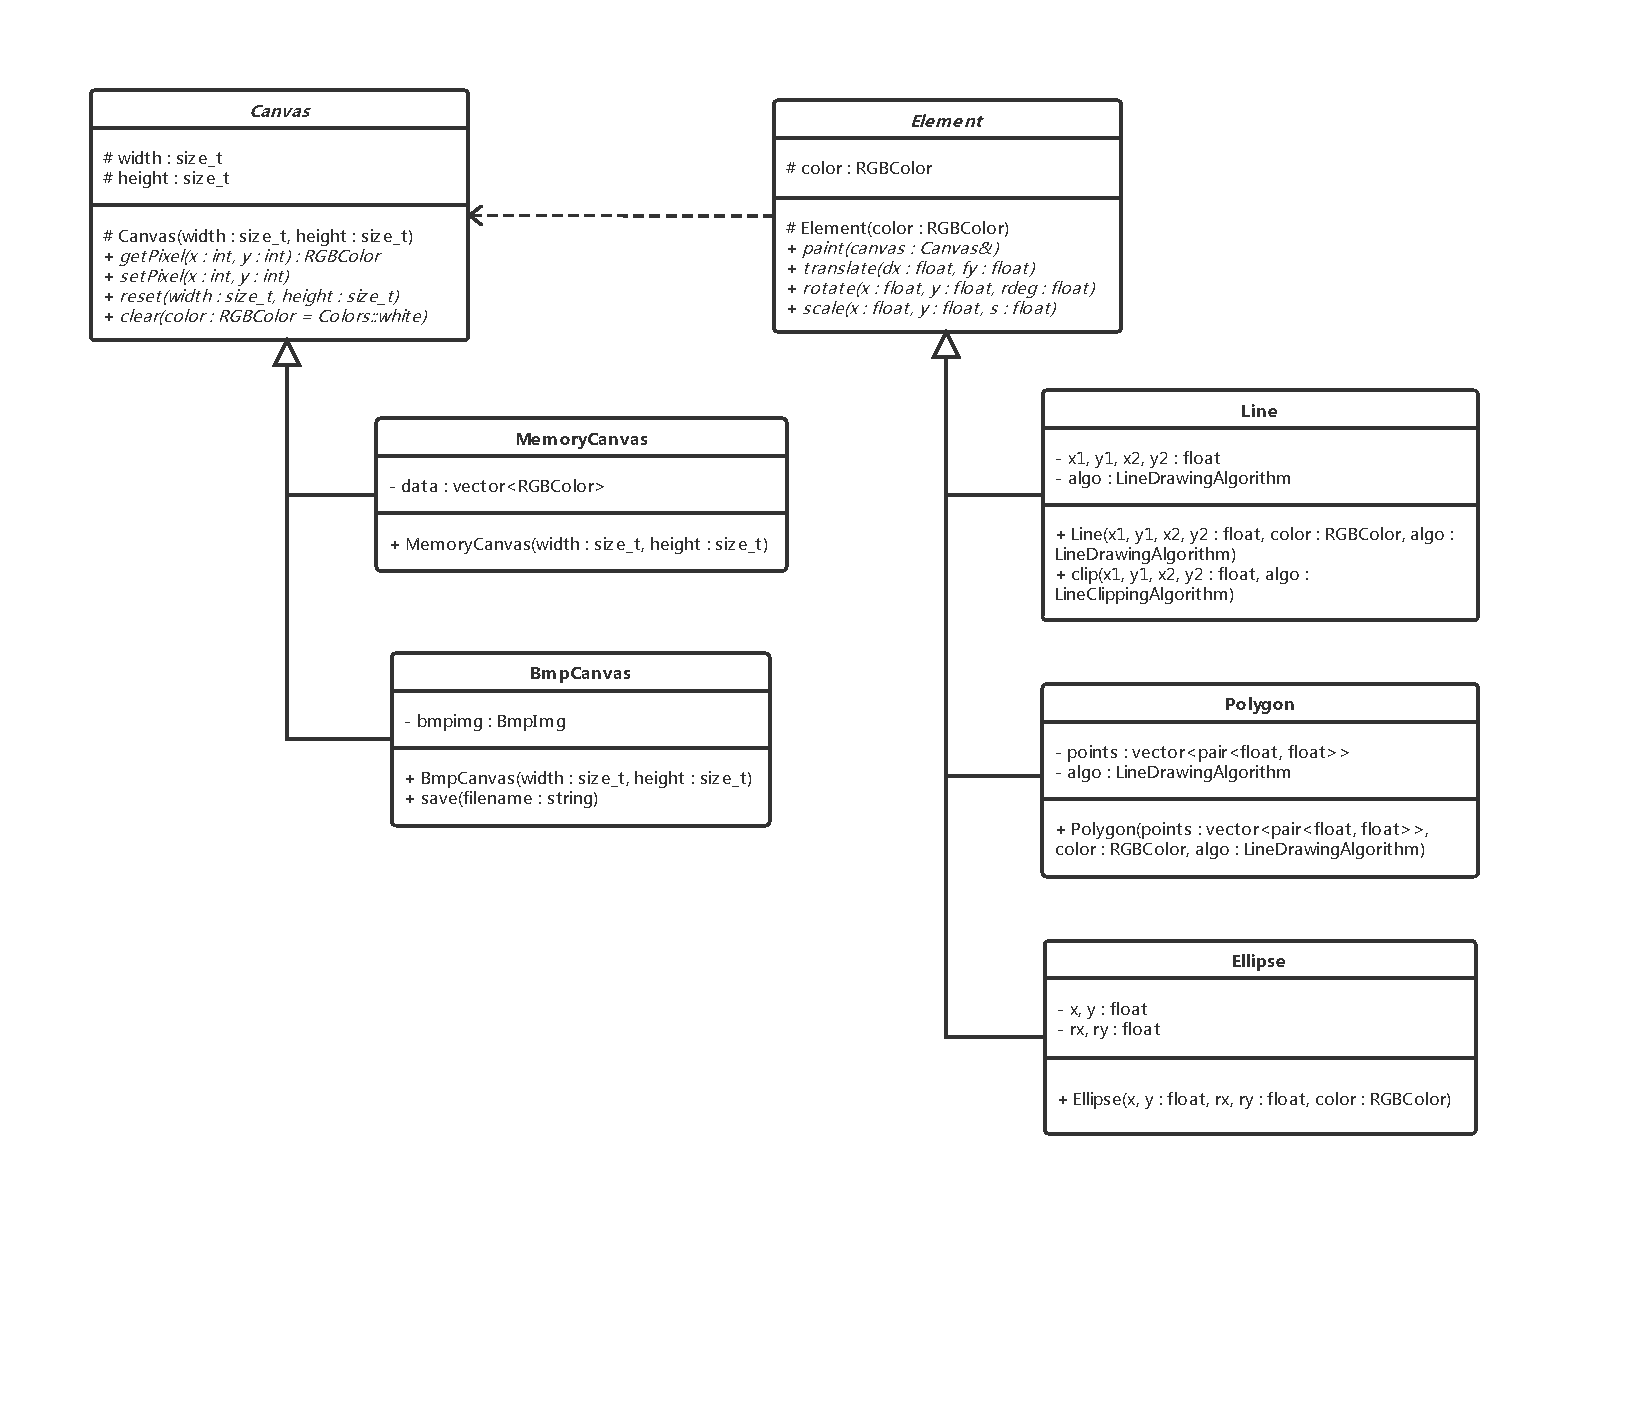
\includegraphics[width=\linewidth]{uml.pdf}
\caption{系统的UML类图}
\end{figure}
\section{总结}
\dots

\bibliographystyle{unsrt}%
%"xxx" should be your citing file's name.
\bibliography{report}
\end{document}
